\documentclass[UTF8,a4paper]{ctexart}

% ==========Preamble==========
\usepackage{graphicx}
\usepackage{apacite}
\usepackage{url}
\usepackage{fancyhdr}
\usepackage{geometry}
\usepackage[font=small,labelfont=bf,labelsep=quad,format=hang,textfont=it]{caption}
\usepackage{booktabs}
\usepackage{graphicx}
\usepackage{float}

\pagestyle{plain}
\CTEXsetup[format=\Large\bfseries]{section}
\bibliographystyle{apacite}
\DeclareGraphicsExtensions{.eps,.pdf,.jpg,.png}

 % 设置图表搜索路径, 可以给图表文件夹取如下名字
\graphicspath{{img/}}

% ==========Title==========

\title{\bfseries Neural Packet Classification论文报告 } 
\author{\bfseries 杨广超\quad202028013229114\\\bfseries 谈昊\quad2020E8013282037}

% Your name in the first blank and your additional information in \thanks{}
\date{\today}
% delete \today if you don't want the date

% ==========Document==========

\begin{document}
\maketitle

% ==========Abstract==========

% \begin{center}
% \parbox{130mm}{\zihao{-5}{\bfseries 摘\quad 要:}
% % Abstract here
% % An example is as follows
% 脑机接口(Brain–computer interface,BCI)是一种可以使人脑与机器产生交流的方法。它使得从大脑发出的信号可以用来控制外部的机器。目前,很多研究兴趣都集中在基于BCI的运动和认知疾病患者的神经康复上。几十年来,BCI已经成为运动和认知康复的一种替代治疗方法。以往的研究表明,BCI干预对恢复运动功能和受损大脑的恢复是有用的。基于脑电图(EEG)的BCI干预可以通过向受损大脑提供反馈,来揭示上肢恢复过程中神经可塑性的机制。BCI可以作为一种有用的工具,在肌萎缩侧索硬化症(ALS)等严重运动丧失病例中,可以帮助患者进行日常的交流和基本的运动。此外,最近的研究结果还报道了BCI对其他不同程度运动障碍疾病患者产生的的治疗效果,如痉挛性脑瘫、神经性疼痛等。除了运动功能恢复外,BCI还在改善注意力缺陷/多动症(ADHD)等认知疾病患者的行为方面发挥了作用。基于BCI的神经反馈训练主要是降低$\theta$ 节律和$\beta$节律的比值,或者使患者能够调节自己的皮质慢速电位,在提高注意力和警觉性方面都取得了进展。通过对多项证据确凿的临床研究的总结,本文介绍了BCI在运动和认知疾病(包括中风、ALS)中的临床应用的前沿成果。
% \par
% \vspace{1mm}
% {\bfseries 关键词:}计算神经科学\quad NLP\quad 实体识别 \quad 知识图谱}
% \end{center}

% ==========Body==========

% Example article

\section{背景介绍}
\subsection{问题描述}
数据包分类一直是计算机网络中的一个基本问题,其目标是在一组规则中,为给定的数据包匹配其中一个规则。数据包分类是许多网络功能的关键组成部分,包括防火墙、访问控制、流量工程和网络测量。因此,数据包分类器的应用十分广泛。在数据包分类过程中,往往需要权衡计算复杂性和状态复杂性。如何缩短分类时间,减少内存占用正是数据包分类问题所面临的难点。
\subsection{研究现状}
现有的数据包分类解决方案可以分为两大类。第一类中的解决方案是基于硬件的,通常利用三元内容寻址存储器(Ternary Content-Addressable Memories,TCAMs)存储所有规则,然后将收到的数据包与这些规则进行匹配。这种方式的分类时间是恒定不变的,但其由于其本身比较复杂,导致了高成本和高功耗。因此,基于TCAM的分类方法很少被用来实现大型分类器。第二类解决方案是基于软件的,一般会构建一个复杂的内存数据结构(通常是决策树)进行数据包分类。此类方案虽然相较比基于TCAM的分类方法具有更大的可伸缩性,但由于分类操作需要从根到匹配的叶遍历决策树,导致其速度更慢。
建立高效的决策树是困难的,经过多年的研究,人们提出了大量基于决策树的数据包分类解决方案但仍然存在两个主要的问题。首先,它们依赖手工调优的启发式来构建树使得它们很难在不同的规则集上理解和优化。其次,这些启发式并没有显式地优化一个给定的目标,而是根据与全局目标联系并不密切的部分信息做决策,这导致其性能可能远远不是最佳的。
目前,将机器学习应用于数据包分类一般有两种方法。第一种方法是用神经网络代替决策树,给定一个数据包,神经网络将输出与该数据包匹配的规则。这种方法的缺点是不能保证总是匹配正确而且评估花费过高。第二种方法,也就是文中作者所采用的方法,即使用深度强化学习(deep reinforcement learning,RL)来建立有效的决策树。

\section{NeuroCuts方法}
\subsection{总体思想}
文章作者设计了一种名为NeuroCuts的深度RL数据包分类方法。给定一个规则集和一个目标函数(例如,分类时间,内存占用,或者两者的组合),通过NeuroCuts学习建立一个决策树,使目标最小化。希望用这样一种基于机器学习的方法来进行数据包分类,从而解决现有手工调优启发式的局限性。
有三个特征使得RL特别适合于数据包分类。首先,构建决策树的解决方案是从一个节点开始,然后反复地对其进行分割。当我们做出割开一个节点的决策时,在我们完成实际树的构建之前,我们不知道这个决策是否是一个好的决策。RL很自然地捕获了这个特性,因为它不假定给定决策对性能目标的影响是立即知道的。其次,不同于现有的启发式,RL算法的明确目标是直接最大化性能目标。第三,能够快速地评估每个模型,显著地减少学习时间。
为了实现这样的设计,作者解决了三个关键的挑战。第一,如何编码变长决策树状态st作为神经网络策略的输入。考虑到到如何分割树中的节点只取决于节点本身,不依赖于树的其他部分,因此,不需要对整个树进行编码,只需要对当前节点进行编码。第二,如何处理在逐个节点构建决策树过程中产生的稀疏和延迟奖励。在这里,作者利用问题的分支结构,为树的大小和深度提供更密集的反馈。第三,如何将解决方案扩展到大型数据包分类器。训练非常大的规则集可能需要很长时间,为了解决这个问题,作者利用了RLlib这个分布式的RL库。
\subsection{主要模块设计}
图\ref{fig:001} 显示了NeuroCuts作为RL系统的结构:环境由规则集和当前决策树组成,而代理使用的模型(由DNN实现)旨在选择最佳的切割或分区操作,以此来增量地构建树。剪切操作将节点按照选定的维度(即SrcIP、DstIP、SrcPort、DstPort和Protocol中的一个维度)划分为若干个子范围(即2,4,8,16或32个范围),并在树中创建这么多的子节点。另一方面,分区操作将一个节点的规则划分为不相交的子集(例如,基于维度的覆盖率),并为每个子集创建一个新的子节点。当前节点的可用操作在每一步都由环境告知,代理在其中选择生成树,随着时间的推移,代理学会优化其决策,以最大限度地从环境中获得回报。图\ref{fig:002} 显示了NeuroCuts的学习过程,其中,x轴表示树的级别,y轴表示该级别上的节点数。树的每一层的切割维度的分布以颜色显示。
	

\begin{figure}[H]
    \centering
    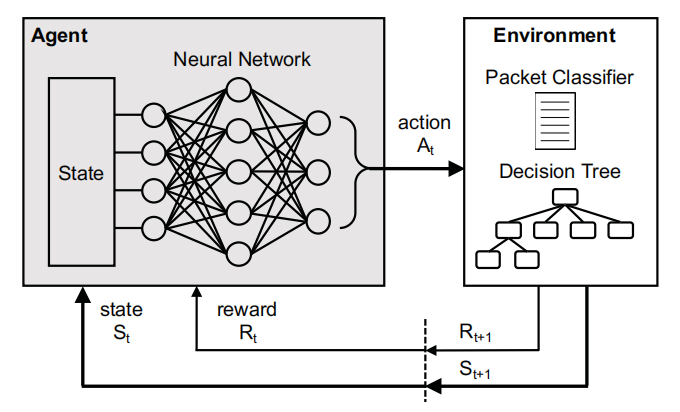
\includegraphics[width = \textwidth]{image001.png}
    \caption{\em NeuroCuts作为RL系统的结构}
    \label{fig:001}
\end{figure}
\begin{figure}[H]
    \centering
    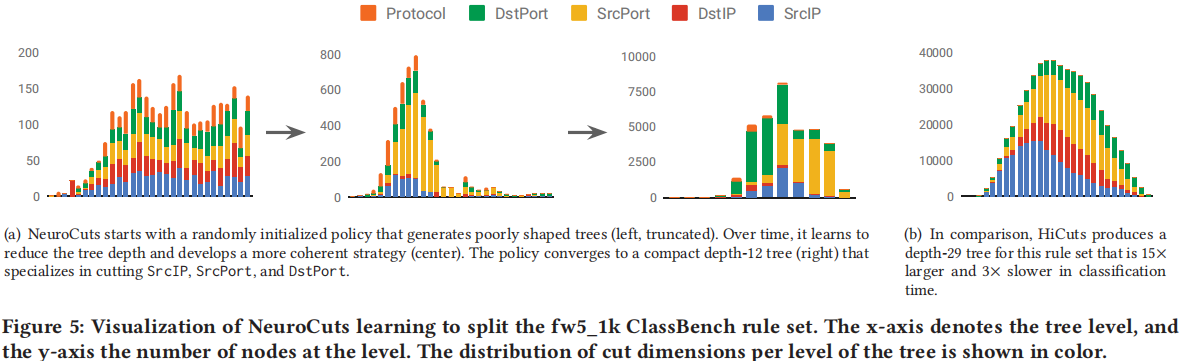
\includegraphics[width = \textwidth]{image003.png}
    \caption{\em NeuroCuts学习分割w5\_1k ClassBench规则集的可视化}
    \label{fig:002}
\end{figure}
\subsubsection{训练算法}
我们使用一个actor-critic算法来训练代理的策略。此算法在许多用例中都提供了较好的结果,并且容易地缩放到分布式环境下。算法1显示了NeuroCuts算法的伪代码,其执行如算法所示。
\begin{figure}[H]
    \centering
    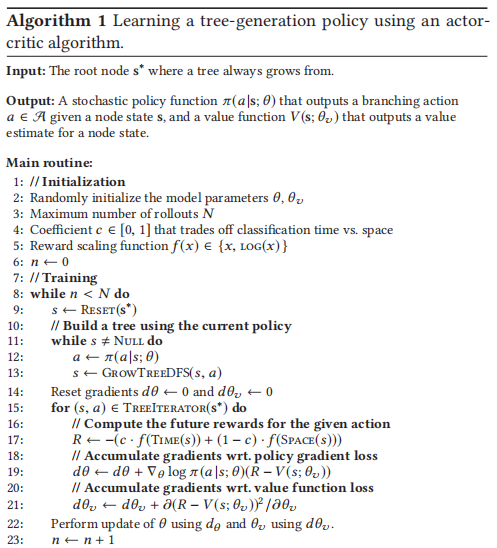
\includegraphics[width = \textwidth]{image005.png}
    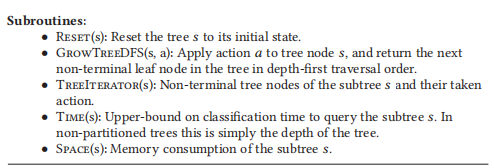
\includegraphics[width = \textwidth]{image007.png}
\end{figure}
\subsubsection{整合现有的启发式}
NeuroCuts很容易加入额外的启发式来改进它学习的决策树,一个例子是添加规则划分动作。除了切割动作,在我们的NeuroCuts实现中,我们还允许两种类型的分割动作:Simple和EffiCuts。
\subsubsection{处理大型包分类器}
小型分类器可以采用NeuroCuts的单线程实现,但对于拥有数万甚至数十万条规则的大型分类器,并行性可以显著提高训练速度。图\ref{fig:003}展示了如何调整算法来并行地构建多个决策树。
\begin{figure}[H]
    \centering
    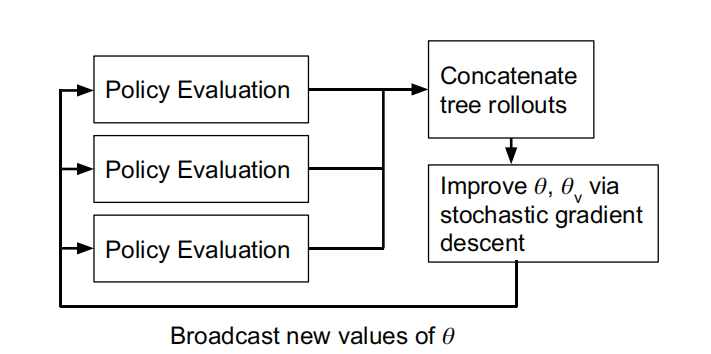
\includegraphics[width = \textwidth]{image009.png}
    \caption{\em NeuroCuts可以通过从当前策略并行生成决策树来并行化}
    \label{fig:003}
\end{figure}
\subsubsection{处理分类器更新}
实际使用过程中经常根据应用需求来更新数据包分类器。对于少数规则的小更新,NeuroCuts修改现有的决策树来反映这些变化,包括添加和删除;当变化较大时NeuroCuts会重新运行训练。
\section{实验评估}
\subsection{实验环境}
在m4.16xl AWS机器上运行NeuroCuts,每个实例使用四个CPU内核加速,使用Python实现决策树的生成,每个NeuroCuts实例最多运行一千万个时间步长,或者直到收敛为止。
\subsection{实验评估}
作者使用标准的ClassBench来生成具有不同特征和大小的数据包分类器,将NeuroCuts与HiCuts、HyperCuts、EfiCuts和CutSplit四种手动调优算法进行比较。基准度量标准包括分类时间和内存占用。结果表明,NeuroCuts在分类时间上显著提高了所有基线,同时也生成了更紧凑的树。在优化内存占用方面,NeuroCuts在不影响时间的情况下,比EffiCuts提高了25\%的中位空间。
在分类时间方面,通过对基于ClassBench分类器的最佳时间优化树的生成时长进行对比,NeuroCuts分别比HiCuts, HyperCuts, EffiCuts和CutSplit提供了20\%,38\%,52\%和56\%的中值改善。
\begin{figure}[H]
    \centering
    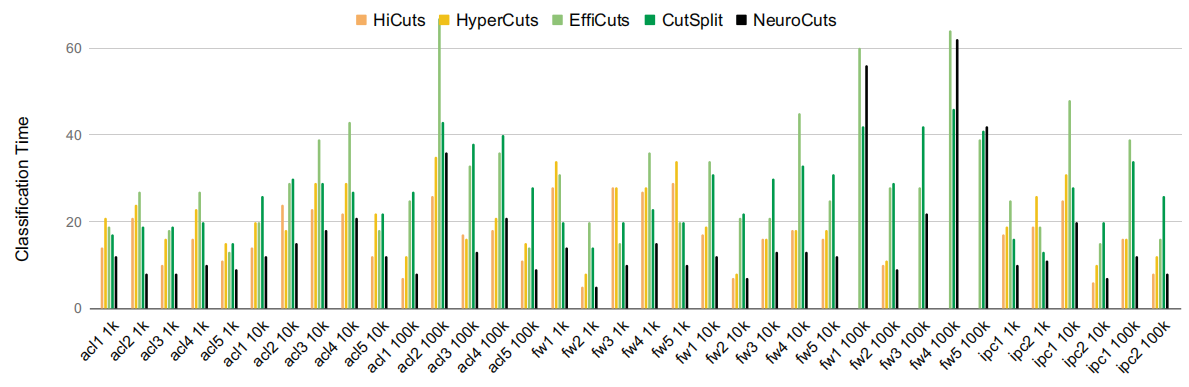
\includegraphics[width = \textwidth]{image011.png}
    \caption{\em HiCuts、HyperCuts、EffiCuts和NeuroCuts的分类时间(树的深度)(时间优化)。我们省略了4个在超过24小时后没有完成的HiCuts和HyperCuts条目。}
    \label{fig:004}
\end{figure}
在内存占用方面,NeuroCuts远远好于HiCuts和HvperCuts,对比EffiCuts,其空间优化树的中值提高了40\%,平均提高了44\%。不过,NeuroCuts与CutSplit相比,中值内存使用量高出26\%,尽管在所有基准上最佳情况下的改进仍然是3倍(66%)。
\begin{figure}[H]
    \centering
    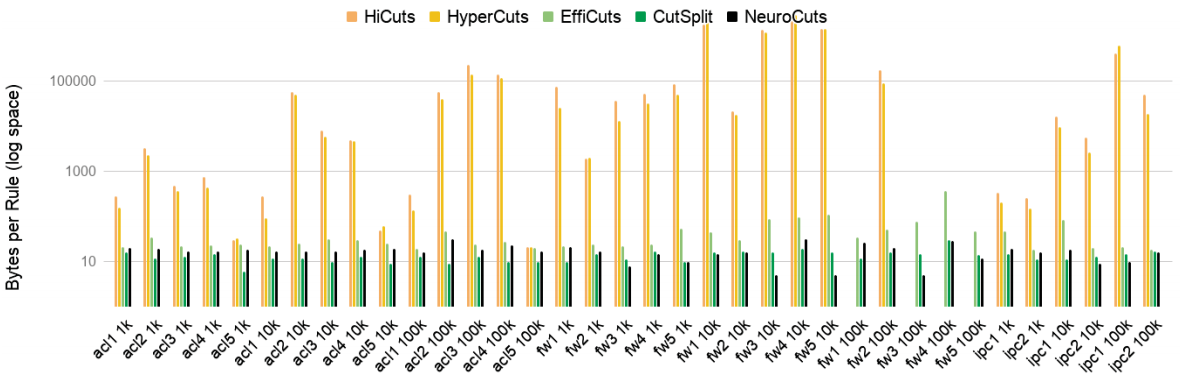
\includegraphics[width = \textwidth]{image013.png}
    \caption{\em HiCuts、HyperCuts、EffiCuts和NeuroCuts(空间优化)使用的内存占用(每个规则的字节数)。我们省略了4个在超过24小时后没有完成的HiCuts和HyperCuts条目}
    \label{fig:005}
\end{figure}
除此之外,实验还表明,NeuroCuts能够有效地合并和改进预先设计的启发式,如EffiCuts顶层划分函数。NeuroCuts可能首先学习产生基本解决方案的随机动作分布,然后利用其神经网络的能力,将动作分布专门化到规则空间的不同部分。最后,作者通过使用简单的分割方法和LOG(X)奖励缩放来扫描NeuroCuts的c值范围发现,时空系数c可以有效权衡并控制内存占用空间和与分类时间。
\begin{figure}[H]
    \centering
    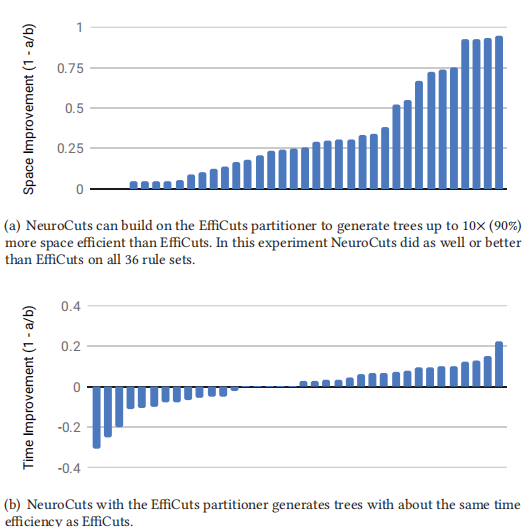
\includegraphics[width = \textwidth]{image015.png}
    \caption{\em 在ClassBench基准测试中,对NeuroCuts相对于效率的改进进行排序。这里只允许使用EffiCuts分区方法运行NeuroCuts。正值表示改进}
    \label{fig:006}
\end{figure}

\begin{figure}[H]
    \centering
    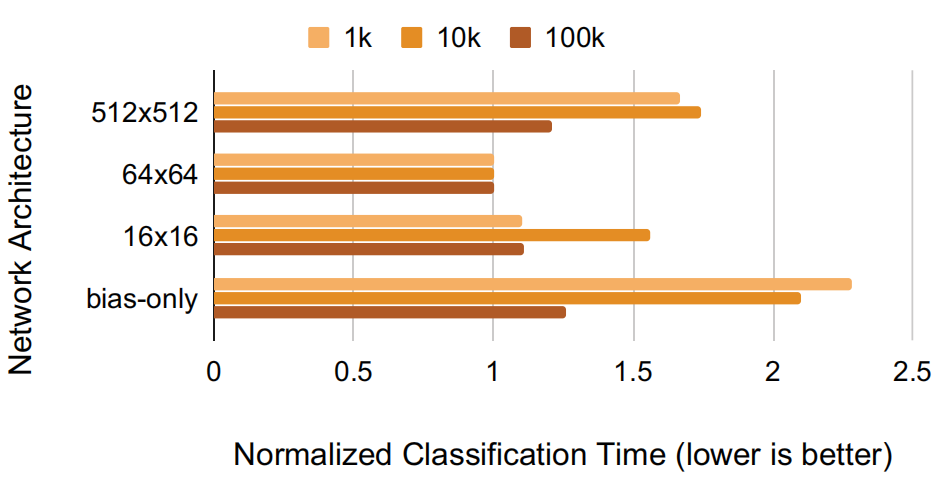
\includegraphics[width = \textwidth]{image017.png}
    \caption{\em 不同网络架构和不同分类器组的神经切割器平均最佳分类时间的比较仅偏倚架构指的是一个不处理观察结果并发出固定动作概率分布(即纯强盗)的普通神经网络。结果在分类器组内进行归一化,使最佳树的归一化时间为1。未收敛到有效树的规则集在归一化之前被分配100的时间}
    \label{fig:007}
\end{figure}
\begin{figure}[H]
    \centering
    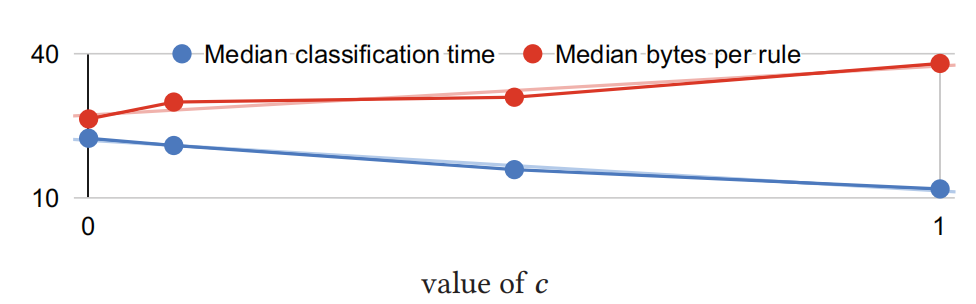
\includegraphics[width = \textwidth]{image019.png}
    \caption{\em 当timespace系数c = 1时,分类时间提高了2x,反之,当c = 0时,每个规则的字节数提高了2x}
    \label{fig:008}
\end{figure}
\section{读后感}
数据包分类应用十分广泛,其难点就在于如何权衡计算复杂性和状态复杂性,尽可能地缩短分类时间,减少内存占用。在这篇论文中,作者基于深度强化学习(RL)方法的三个重要特征,创造性地建立了NeuroCuts来解决数据包分类问题。实验评估表明,相较目前几种手动调优算法,这一系统在分类时间和内存占用空间等方面都取得了非常不错的表现。
\par
强化学习一般用于描述和解决智能体在与环境的交互过程中通过学习策略以达成回报最大化或实现特定目标的问题,在信息论、博弈论、自动控制等领域都得到了广泛的讨论。这篇文章的作者将其应用于数据包分类领域并取得了良好的效果,为解决包分类问题提供了一个新的思路。\par
通过阅读这篇文章,我们全面地了解了数据包分类问题的研究现状以及难点,明确了该领域当前面临的困境及应重点突破的方向。此外,我们还进一步加深了对深度强化学习的理解,尤其是在研究RL适用于数据包分类的三个特征以及NeuroCuts设计过程中的三个挑战和解决方案的过程中,我和我的队友就RL能解决什么问题以及如何使用RL解决问题进行了深入的思考与讨论。进一步认识RL奖励的延迟和稀疏两个特点以及学习如何将可变长度决策树状态编码为神经网络策略的输入将会对我们将来的学习与科研有所启发。
\section{作者背景介绍}
\begin{itemize}
    \item Eric Liang:加州大学伯克利分校RISELab成员之一,方向为强化学习的分布式系统和应用程序,曾在Google/Databricks工作。
    \item Ion Stoica:加州大学伯克利分校EECS系的教授,RISELab成员之一。他从事云计算和网络计算机系统的研究,也是ACM院士。
    \item Hang Zhu:约翰·霍普金斯大学计算机科学系的博士研究生,毕业于清华大学,是Xin Jin的学生,从事计算机网络的研究。
    \item Xin Jin:约翰霍普斯金大学计算机系的助理教授,曾在加州大学伯克利分校AMPLab/RISELab工作,从事计算机网络和分布式系统领域的研究。
\end{itemize}
本文作者来自伯克利的RISElab(\url{https://rise.cs.berkeley.edu/})。RISELab代表着实时智能安全执行(RISE),其定位是在分布式计算中解决下一个阶段,根据Databricks博客的说法:“Storica曾表示,这个新阶段是为了通过两个项目——Drizzle和Opaque,改进Spark并实现创新,其致力于构建开源框架、工具、算法,以便能够以更高的安全性,根据实时数据,决定要构建哪些实时应用。”

RISELab的初期目标是为了增强Spark的安全性与实时能力,因此,根据Databricks的信息,Drizzle项目的目标是将Spark Streaming的延迟降低一个数量级,同时提高其容错性。Opaque项目是为了增强Spark的动态与静态数据的加密功能。

\clearpage


\end{document}
